\section{Resource Allocation} \label{sec:decompose}

The output of the transformation (\Cref{sec:control}) is a VUDFG that 
can execute on a Plasticine with infinite-sized physical units (PUs).
The \emph{Resource Allocation} phase enforces and addresses constraint violations given 
the specification of the Plasticine units. 
At the end of this phase, \name assigns each VU in the VUDFG graph to a PU type with required
resources; the placer then takes the type assignments and determines the final placement.

Accelerators often have heterogeneity in compute resources to improve efficiency for commonly used
special operations.
In Plasticine, PMUs and DAGs have specialized compute pipelines for address calculation that are 
less capable than the compute pipeline in PCUs.
However, heterogeneity tends to reduce average utilization because different applications, and even the same
application with different data sizes, can vary highly in the desired ratio among different resource.
A compute-bound application, for example, can heavily underutilize the DAGs and PMUs.
To address this problem, \name models the virtual to physical assignment as a constraint satisfaction problem; 
each VU consumes a set of resources and can only be assigned to a PU if the PU processes the required resources. 
%Instead of using heuristics to assign certain a type of VU to a type of PU, we
\Cref{tab:resource} shows the types of resources in Plasticine's heterogeneous units.
For example, special connection to off-chip memory interface is
also treated as a type of resource in the DAG, which forces virtual contexts accessing DRAM to map to DAGs. 
On the other side, regular contexts with non-vectorized fixed-point operations can also be mapped to
spare DAGs, which improves utilization.
\begin{table*}
  \centering
\begin{tabular}{lcccc}
  \toprule
  Feature & PCU & PMU & DAG & Host Unit\\ \midrule
  Vector lane width & 16 & 16 & 1 & 1 \\
  Fixed-point op & \cmark & \cmark & \cmark & \xmark\\
  Float-point op & \cmark & \xmark & \xmark & \xmark\\
  Number of stages & 6 & 10 & 5 & 0 \\
  Number of pipeline registers & 8 & 8 & 4 & 0 \\
  Reduction tree & \cmark & \xmark & \xmark & \xmark\\
  \# Vector FIFO & 6 & 6 & 4 & 0\\
  \# Scalar FIFO & 6 & 6 & 4 & 16\\
  \# Control FIFO & 16 & 16 & 4 & 16\\
  Scratchpad banks & 0 & 16 & 0 & 0 \\
  Scratchpad capacity & 0 & 256kB & 0 & 0\\
  MergeBuffer & \cmark & \xmark & \xmark & \xmark\\
  Splitter & \cmark & \xmark & \xmark & \xmark\\
  Scanner & \cmark & \xmark & \xmark & \xmark\\
  Access to DRAM Interface & \xmark & \xmark & \cmark & \xmark \\
  Access to Host IO & \xmark & \xmark & \xmark & \cmark \\
 \bottomrule
\end{tabular}
\caption[Mapping between data-structure to hardware memories]{
  MergeBuffer, Splitter, and Scanner are new hardware introduced in \cite{gorgon} and \cite{capstan}
  to support database and sparsity in Plasticine.
}
\label{tab:resource}
\end{table*}

\begin{algorithm}
  \Fn(\tcc*[h]{Allocation Algorithm}){alloc(V, P, pruners)}{
    \KwData{V: a set of VUs from the VUDFG}
    \KwData{P: a set of all PUs on the hardware}
    \KwData{pruners: a list of constraint pruners to check
    and fixes constraint violations}
    \tcc{Initialize a complete bipartite graph}
    G = \KwNew BipartiteGraph()\;
    G[V] = P\;
    \tcc{Constraint resolution}
    prune(G, pruners)\;
    \tcc{Global merging}
    merge(G)\;
    \tcc{Heuristic check on whether assignment is feasible}
    check(G)\;
    \tcc{Virtual to physical assignment}
    backtracking\_assign(G)\;
  }
  \vspace{0.5cm}
  \Fn(\tcc*[h]{A recursive pruning function}){prune(G, pruners)}{
    \KwData{G: bipartite graph between VUs and PUs}
    \KwData{pruners: a list of constraint pruners to check
    and fixes constraint violations}
    \KwResult{The function update G by removing VU-PU edges that violates constraints guarded by
    pruners. The function may fail and raise an exception.}

    \For{pruner \KwTo pruners}{
      \For{v \KwTo G.keys()}{
        \For{p \KwTo G[v]} {
          \If{!pruner.fit(v,p)} {
            G[v] -= p\;
          }
        }
        \If{G[v].empty()} {
          \tcc{Partition VU v based on resource constraints registered in pruner. 
          Not all resources can be partitioned and this step may fail.
          If succeeded, the function returns a new set of VUs.}
          V' = pruner.partition(v)\;
          G' = \KwNew BipartiteGraph()\;
          G'[V'] = G.values()\;
          prune(G',pruners)\;
          G -= v\;
          G[V'] = G'[V']\;
        }
      }
    }
  }
  \caption{Resource allocation. The bipartite graph \texttt{G} contains a bi-directional many-to-many
  map. \texttt{G[key]} returns a set of values, and \texttt{G[value]} returns a set of keys.
  \texttt{G[KeySet] = ValueSet} creates all-to-all assignment between \texttt{KeySet} and
  \texttt{ValueSet}.}
  \label{algo:resalloc}
\end{algorithm}

\begin{algorithm}
  \Fn(\tcc*[h]{Assignment feasibility check}){check(G)}{
    \KwData{G: bipartite graph}
    \KwResult{whether assignment is possible}
    \tcc{For every value set in \texttt{G}}
    \For{V \KwTo G.values().toSet()} {
      K = $\emptyset$\;
      \For{v \KwTo V} {
        \For{k \KwTo G[v]} {
          \If{G[k] $\subset$ V} {
            K += k\;
          }
        }
      }
      \If{|K| > |V|} {
        \KwRet{failure()}\;
      }
    }
    \KwRet{success()}\;
  }
  \caption{Heuristic check on whether it is possible to assign all key with an value in a bipartite
  graph. Given there are only a few types of hardware tiles, $G.values().toSet()$ is
  relatively small. This algorithm roughly runs in $O(|G.keys()|\times|G.values()|)$, which is
  still much faster than the backtracking assignment, which has exponential runtime.}
  \label{algo:check}
\end{algorithm}
 
%% backtracking_assignment(vu, dom)
As shown in \Cref{algo:resalloc}, the \emph{resource allocation} phase contains three steps:
\emph{constraint resolution}, \emph{global merging}, and \emph{virtual to physical assignment}.
\name uses a VU-PU bipartite graph (\texttt{G}) to keep track of potential valid assignments between the two.
Initially, \texttt{G} is initialized to a complete bipartite graph, i.e. all VUs can be assigned to
all PUs.

\paragraph{Constraint Resolution}
A list of constraint pruners, each considering a set of on-chip resources, 
incrementally remove the VU-PU edges that violate the resource constraints.
If a VU \texttt{v} has no mappable PU after pruning, the pruner attempts to fix the violation by
decomposing the VU into multiple VUs. 
Not all resources can be composed and the partitioning transformation may fail.
If succeeded, the partitioner generates a new set of VUs \texttt{V'}. \name starts a new complete bipartite
graph between \texttt{V'} and all resources \texttt{P}, and recursively prune on \texttt{V'}.
If succeeded, the original graph \texttt{G} is updated with \texttt{V'} and their pruned resources.

\paragraph{Global Merging}
After all VUs have at least one PU in the bipartite graph, \name triggers a global optimization that merges 
small VUs into a larger VU to reduce fragmentation in allocation.
Each type of resource has an aggregation rule to compute how the resource usages change if two VUs are merged
together. Most aggregation rules are simple, such as addition, logical or, max, or union.
The in- and out-degree increases are tricker and will be detailed in \Cref{sec:compsplit}.

\paragraph{Virtual to Physical Assignment}
Next, \name performs a quick heuristic check on the bipartite graph to see if there exists a
possible assignment for all VUs with sufficient PUs (\Cref{algo:check}), and provide feedback on the
limiting resources, otherwise.
Finally, \name assigns each VU to a PU type with a backtracking search on the pruned bipartite
graph.

This approach can be easily extended to handle new heterogeneous tiles in the architecture by registering
new types of resources with aggregation and partitioning rules.
The rest of this section will focus on two types of partitioning transformations--compute
partitioning in \Cref{sec:compsplit} and memory partitioning in \Cref{sec:memsplit}.
%We have another partitioner encoding valid rule to decompose a BlackBox IP block available on the RDA.

\subsection{Compute Partitioning} 
\label{sec:compsplit}

The {\em compute-partitioning} phase addresses VUs using more compute resource than any PU can provide. 
If a VU contains multiple contexts, \name{} first moves the contexts into separate VUs.
If a single context exceeds the resource limit, \name breaks down the dataflow graph in the context into 
multiple contexts and put them in separate VUs.
During partitioning, \name maps each subgraph of the large dataflow graph into a new context, 
mirrors the control states of the original context, and streams live variables in between.
We can formulate the problem of how to partition in the dataflow graph as an optimization problem, shown in
\Cref{tab:partprob}.
The partitioner ``fixes'' the VU \texttt{v} based on a single PU specification, albeit there are many potential PUs 
the decomposed VU can be mapped to.
Currently, we use a heuristic to select a PU type from \texttt{G[v]} right before the compute pruning 
as a guiding constraint for partitioning.

\begin{table*}
  \centering
\begin{tabular}{lp{12cm}}
  \toprule
  \textbf{Problem} & Partition the dataflow graph into subgraphs such that all subgraphs satisfy the constraints of a
  hardware unit. \\[0.9cm]
  \textbf{Objective }& Minimize the number of partitions and connectivity across partitions. \\[0.5cm]
  \textbf{Constraints} & 
  \begin{minipage}{12cm}
  \begin{outline}
  \0 Each partition must not exceeds the limit on the number of \vspace{-0.2cm}
    \1 live in/out variables (I/O ports) \vspace{-0.2cm}
    \1 operations (pipeline stages), \vspace{-0.2cm}
    \1 and live variables across operations (pipeline registers), etc.\vspace{-0.2cm}
  \0 No \emph{new} cycles can be formed across partitions other than the cycles in the original
  dataflow graph.
  \end{outline}
  \end{minipage}
  \\
 \bottomrule
\end{tabular}
\caption[Formulation of the compute partitioning problem]{
Formulation of the compute partitioning problem
}
\label{tab:partprob}
\end{table*}

Because the global network is specialized to handle efficient broadcasts, 
the in/out-degree of a partition counts the number of unique live-in/out variables, as supposed to
number of edges across partitions.
In addition, the partitioned subgraphs cannot form {\em new} cycles; contexts waits for all
input dependencies and therefore cycles across contexts cause deadlock. 
Nonetheless, the original graph might contain cycles representing loop carried dependencies, such as
accumulation. For these cycles, \name initialize the back edge of the cycle with dummy data to
enable execution.
\Cref{fig:parteg} shows examples of valid and invalid partitioning solutions.

\paragraph{Community Detection}
The formulation of compute partitioning is similar to the community detection problem\cite{community}, which has similar
objective. The major difference is that the later often takes the number of output partitions as an
input to the algorithm, whereas our problem partitions until all subgraphes satisfy all constraints.
Moreover, community detection algorithms do not enforce the cycle constraints. 
Finally, the edge connectivity in community detection counts the number of edges across partitions, as supposed to broadcast edges.

\paragraph{Retiming}
Imbalanced data paths across partitions can cause pipeline stalls at runtime.
To ensure full-throughput pipelining, \name needs to insert retiming buffers along imbalanced data path across
partitions.
Retiming introduces new VUs in addition to the partitioned VUs, which attributes to the cost in
\Cref{tab:partprob}'s objective.

In the following sections, we present two algorithms to solve this problem--
a traversal-based algorithm providing a decent solution with fast compile time, and a convex
optimization-based algorithm with an optimum solution but long compile time.

\begin{figure}
  \centering
  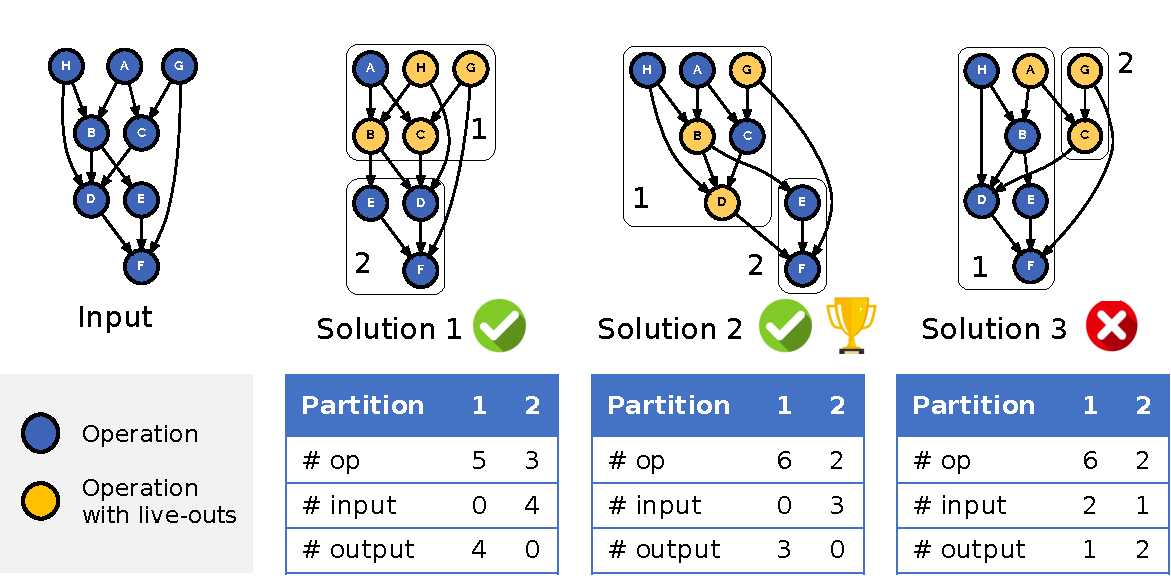
\includegraphics[width=1\columnwidth]{figs/parteg.pdf}
  \caption[Compute partitioning examples]{
    Compute partitioning examples. Solution 1 and 2 are both valid partitioning. Solution 2 is
    better because it has less number of broadcast edges across partitions. Solution 3 is an example
    of illegal partition result due to the cycle between partition 1 and 2.
  }
  \label{fig:parteg}

  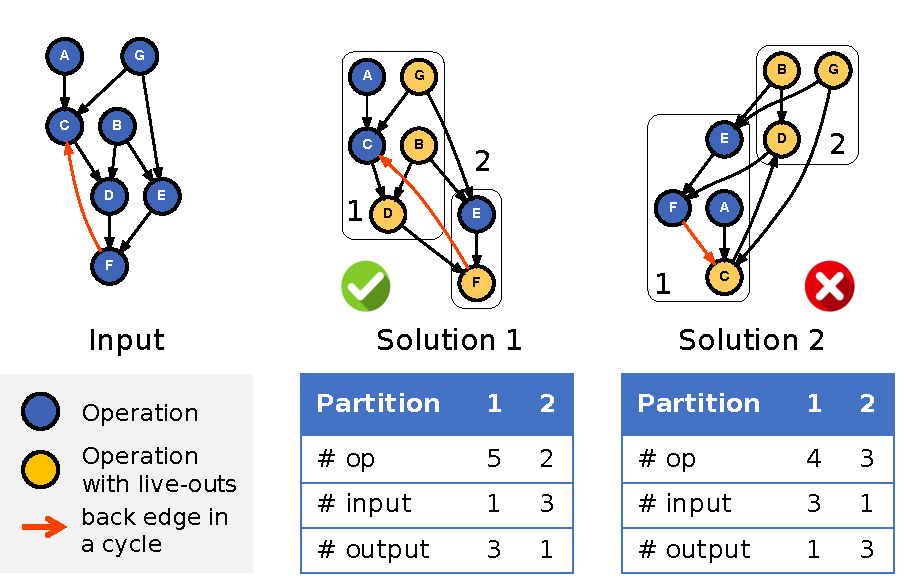
\includegraphics[width=0.8\columnwidth]{figs/partcycleeg.pdf}
  \caption[Compute partitioning examples with cycle]{
    Compute partitioning examples with cycle in the dataflow graph.
    Solution 1 is valid because there is no 
    cycle between partitions after removing the back edge in
    the original graph in Solution 1. 
    Solution 2 is invalid because there is still cycle between partition 1 and 2 after
    removing the original back edge.
  }
  \label{fig:parteg}
\end{figure}

\subsubsection{Traversal-based Solution}
The traversal-based solution iteratively adds nodes to a partition until the partition can fit no
more nodes.
To address the cycle constraint, we perform a topological sort of the dataflow graph.
The topological traversal ignores the back-edge of the cycles during traversal. 
The compiler starts from the beginning of the list, recursively adds nodes into a partition until the partition no longer satisfies the hardware constraint, and repeats the process with a new partition.
This approach guarantees that no cycle is introduced with $O(V+E)$ complexity, where $V$ and $E$ are the numbers of vertices and edges.
However, the outcome of the partitioning is a function of the traversal order, which does not guarantee an optimum solution, which we experienced with depth-first search (DFS) and breadth-first search (BFS) with forwarding and backward traversals.
For DFS, we re-sort the remaining list each time we start with a new partition.

%The forward traversal schedules nodes as earlier as possible, which reduces the number of
%external live variables and the backward traversal minimizes the number of internal variables.
%The DFS minimizes the number of live variables between partitions, albeit producing more imbalanced paths between
%partitions. On the other hand, BFS produces more balanced partitioning with more live variables and partitions.

\subsubsection{Solver-based Solution}
\Cref{tab:solver-eqns} gives our formulation of the partitioning problem.
At a high-level, we use a boolean matrix $B$ to keep track of the assignment of nodes in the dataflow graph to partitions. 
$B$ has dimension of number of nodes to number of partitions, where$B[i,j]==1$ indicates an assignment of node $i$ to partition $j$. 
Each node is constrained to have a single partition assignment.
The input and output arity constraints show the formulation of the PU I/O constraints.
These are the two most challenging constraints as we need to identify broadcast edges across partitions.
To address the cycle constraint, we introduce a delay vector $d$ with size equal to the number of nodes. 
The delay vector encodes a schedule to execute each node. 
A node cannot execute earlier than its input dependencies and cannot be scheduled later than its output dependencies (Delay Consistency).
The dependency constraint further limits nodes belonging to the same partition to have the same delay.
This delay variable is also used to calculate where retiming is required and projection of the amount of retiming VUs introduced. 
The final object is just the sum of partitioned VUs and retiming VUs.
To limit $B$ to a small size, we use the traversal solution to determines the initial column size of $B$.

\begin{table*}
  \centering
	\begin{tabular}{c | c | c | c}
		\textbf{Name} & \textbf{Type} & \textbf{Description} & \textbf{Definition / Default}\\\hline
		$\mathcal{N}$ & Constant & Enumeration of nodes to partition, numbered $\{n_i\}_i$ & - \\
		N & Constant, $\nnint$ & Number of operations to partition & $N = |\mathcal{N}|$\\
		P & Constant, $\nnint$ & Number of partitions to consider & $N$, or from heuristic \\
		$\mathcal{E}$ & Constant, $\{n_i \to n_j\}$& Directed edges representing dependence & - \\
		B & Variable, $\{0, 1\}^{N \times P}$ & Boolean Partitioning Matrix& - \\
		%p & Variable, $\nnint^N$ & Vector of mappings from node to assigned partition& $p = B \begin{bmatrix} 0 & 1 & \cdots & P-1\end{bmatrix}^T$\\
		$\projb{\cdot}$ & $\nnint \to \mathbb{B}$ & Function to convert a positive integer into a boolean& Supplemental Materials\\
		$\andf(\cdot, \cdot)$ & $\{0, 1\} \times \{0, 1\} \to \{0, 1\}$ & Boolean and of binary variables & Supplemental Materials \\ 
		$d_p$ & Variable, $\nnint^P$ & Vector of partition delays & - \\
		$d_n$ & Variable, $\nnint^N$ & Vector of node delays & - \\
		$\dest(n)$ & $\mathcal{N} \to \mathcal{P}(\mathcal{N})$& The set of nodes which depend on $n$& $\{n' | n' \in \mathcal{N}\ s.t.\ (n \to n') \in \mathcal{E}\}$\\
		$c_o$ & Constant, $\nnint$ & Maximum output arity of a partition & HW Spec \\
		$c_i$ & Constant, $\nnint$ & Maximum input arity of a partition & HW Spec \\
		$b_d$ & Constant, $\nnint$ & Maximum input buffer depth & HW Spec \\
		$K$ & Constant, $\mathbb{R}_+$ & Very Large Constant, used for constraint activation & $P \times N$ \\
		$\alpha_d$ & Hyperparameter, $\mathbb{R}_+$ & Retime merging probability multiplier& $\frac{1}{\max\{c_o, c_i\}}$ \\
	\end{tabular}
	\caption{Names and definitions used in the solver-based partitioning.}
	\label{tab:solver-variables}
\end{table*}

\begin{table*}
  \centering
  \newcommand\cola{1.6cm}
  \newcommand\colb{3.8cm}
  \newcommand\colc{9cm}
  \newcommand{\gcell}[2]{\Gape[#1cm][0cm]{\makecell[l]{#2}}}
  \begin{tabularx}{\textwidth}{cp{\colb}X}
    \toprule
		\textbf{Type} & \textbf{Description} & \textbf{Expression}\\\midrule
    \multirow{3}{*}{\makecell[l]{Cost\\Function}} & Allocated Partitions & $\Sigma_i \projb{\Sigma_j B_{i, j}}$\\

    & \makecell[l]{Additional Retiming\\Partitions}
    & $\alpha_d \Sigma_{n_i \to n_j \in \mathcal{E}} \projb{\max\{d_n(j) - d_n(i) - b_d, 0\}}$\\[0.3cm]
		\hline

    \multirow{12}{\cola}{\makecell[l]{\\\\Constraint}} & Partition Assignment & $ \forall n_i \in \mathcal{N}:\ \Sigma_j B_{i, j} = 1$\\[0.1cm]

    &\makecell[l]{Dependency\\Constraint} & $\forall n_i \to n_j \in \mathcal{E}:\ d_n(i) + 1[p_i \ne p_j] \le d_n(j)$\\[0.1cm]

    &\makecell[l]{Output Arity\\ Constraint} 
    &\makecell[l]{
      $\forall p \in [0, P):$ \\
      $\Sigma_{n_s \in \mathcal{N}} \andf(B_{s, p}, \projb{\max\{(\Sigma_{n_d \in \dest(n_s)} B_{d, p}) -$ \\
      $K \times B_{s, p}, 0\}}) \le c_o$
    }\\[0.7cm]

    &\makecell[l]{Input Arity Constraint\\ (vectorized)} & $\Sigma_{n_i \in \mathcal{N}} \max\{\projb{\Sigma_{n_j \in \dest(n_i)} B_{j, :}} - B_{i, :}, 0\} \le c_i \times \vec{1}$\\

		&Delay Consistency& 
    \makecell[l]{
    $\forall n_i \in \mathcal{N}:\ d_n(i) \le \min_j (d_p(j) + K - B_{i, j} \times K)$ \\
		$\forall n_i \in \mathcal{N}:\ d_n(i) \ge \max_j (d_p(j) + B_{i, j} \times K - K)$
    }\\[0.5cm]

		&Constant Validity& 
    \makecell[l]{
      $\forall n_i \in \mathcal{N}:\ d_n(i) \le K$\\
		  $\forall i \in [0, P):\ d_p(i) \le K$
    } \\
    \bottomrule
	\end{tabularx}
  \caption{Solver formulation for partitioning*.}
	\label{tab:solver-eqns}
\end{table*}

\begin{table*}
	\begin{tabular}{c | c | c | c}
		\textbf{Name} & \textbf{Type} & \textbf{Description} & \textbf{Definition / Default}\\\hline
		$\mathcal{C}_r$& $[\mathcal{N} \to \mathbb{R}_+,\mathbb{R}_+, [\mathbb{R}_+] \to \mathbb{R}_+]$ & List of per-node values, limits, and reduction& Supplemental Materials\\&& functions for reducible constraints& \\
		F & $\{0, 1\}^{N \times P}$ & Feasibility matrix, whether a partition can support a node& HW Spec \\ 
	\end{tabular}
	\caption{\Cref{tab:solver-variables} extension for solver-based merging, which is a generalization of the partitioning problem.}
	\label{tab:merging-variables}

	\begin{tabular}{c | c | c}
		\textbf{Type} & \textbf{Description} & \textbf{Expression}\\\hline
		Constraint & Feasibility Constraint & $ \forall i, j \in [0, N) \times [0, P):\ B_{i, j} \le F_{i, j}$\\
		& Reducible Constraints & $\forall j \in [0, P).\ \forall (c(\cdot), c_v, r(\cdot)) \in \mathcal{C}:\ r([c(n_i) \times B_{i, j}]_{n_i \in \mathcal{N}}) \le c_v$\\
	\end{tabular}
  \caption{\Cref{tab:solver-eqns} extension for solver-based merging*. The Retiming Partition objective is not used for merging.}
	\label{tab:merge-eqns}
  \scriptsize
  \raggedright
  \vspace{-0.3cm}
  *Expressions are presented using the Disciplined Convex Programming ruleset \cite{DCP, DCP-online}. Explanations for selected expressions can be found in the supplemental material.
\end{table*}



\begin{figure*}
\centering
\hfill
\begin{subfigure}[b]{0.35\textwidth}
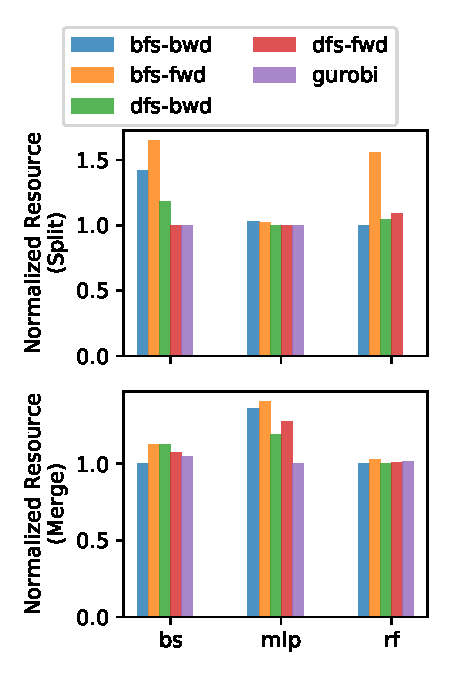
\includegraphics[width=1\textwidth]{figs/algo2.pdf}
\caption{Resource Comparison}
\end{subfigure}
\hfill
\begin{subfigure}[b]{0.64\textwidth}
\centering
\begin{tabular}{lccccc}
  \toprule
  Apps &bfs-bwd & bfs-fwd & dfs-bwd & dfs-fwd & gurobi \\ \midrule 
bs & 3s & 3s & 2s & 2s & 2h4m \\ 
mlp & <1s & <1s & <1s & <1s & 4s \\ 
rf & 1m37s & 1m7s & 29s & 27s & - \\ 

 \bottomrule
\end{tabular}
\caption{
  Compile time for spltting
}
\vspace{0.1cm}
\begin{tabular}{lccccc}
  \toprule
  Apps &bfs-bwd & bfs-fwd & dfs-bwd & dfs-fwd & gurobi \\ \midrule 
bs & 1s & 2s & 5s & 3s & 1m4s \\ 
mlp & 5s & 5s & 6s & 11s & 31m16s \\ 
rf & 11s & 10s & 2m7s & 1m0s & 14h27m \\ 

 \bottomrule
\end{tabular}
\caption{
  Compile time for merging
}
\vspace{0.65cm}
\end{subfigure}
\hfill
\caption[Partitioning and merging algorithm comparisons]{
  Partitioning and merging algorithm comparisons. (a) shows the normalized resource usage between
  different algorithms (the lower the better). (b) and (c) shows the compile time of each algorithm.
}
\label{fig:split}
\end{figure*}

\subsection{Memory Partitioning} \label{sec:memsplit}
The memory pruner addresses VUs with virtual on-chip scratchpad memories exceeding the physical limits in capacity or number of banks in a PU.
Memories in the input graph can have arbitrary size and number of virtual banks.
The PUs, on the other hand, contains a small number of fix-sized 1-D scratchpad banks.

To partition the virtual memory, \name{} shards the large virtual memory into multiple memory partitioned VUs, and assign each partition with a subset of the virtual banks.
Each accessor provides a bank ID (BI) that selects which banks to access and a bank offset (BO) that specifies the address within the bank. 
BI and BO can be vectorized.
\name{} can use multiple banks within a PU to form a larger virtual bank.
However, if a virtual bank in VU exceeds the total capacity of all physical banks within a PU, \name{} further partitions the large virtual banks into multiple sub-banks, such that each sub-bank can fit into the aggregated capacity of a PU.
To do so, \name{} injects additional calculation to derive the sub-bank ID and sub-bank offset from the BO, and flattens the sub-bank ID with the previous BI to form the new BI and the new BO.

%The number of banks required in VU increases with parallelization of the program to increase memory access bandwidth.
%The memory is further multi-buffered to enable coarse-grained pipelining across loop nests\cite{sptial}.
%The total amount of banks required is the product of the number of banks along all dimensions.
%The capacity per bank is the capacity of the logical memory divided by the number of banks.

\begin{figure}
  \centering
  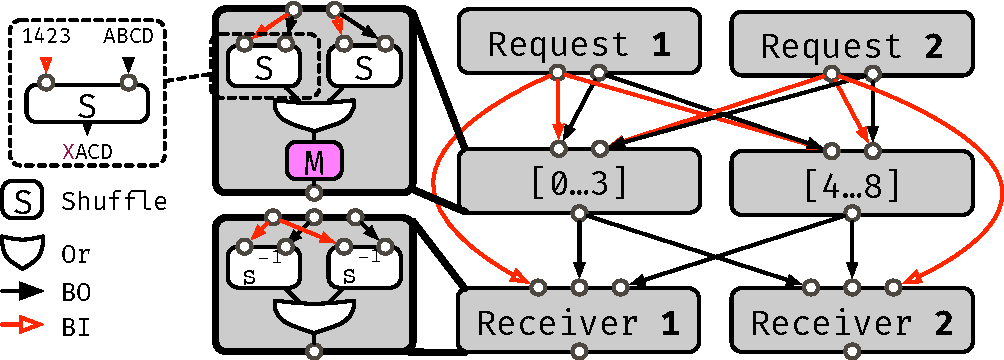
\includegraphics[width=1\columnwidth]{figs/memsplit.pdf}
  \caption{An example of splitting a memory to serve parallel requesters.}
  \label{fig:memsplit}
\end{figure}

\name{} then set ups the crossbar data path between the parallel producers, memory partitions, and parallel consumers.
As discussed in \Cref{sec:sync}, each accessor is split into a requester context and receiver context.
For each memory partition, \name{} uses an context to merge the requests from all parallel requesters, \Cref{fig:memsplit}.
The merge context uses a special shuffle operator that shuffles the BO vector from the order in BI to the order aligned with banks in its partition.
If a bank in the partition is not accessed in BI, the output of the shuffle is marked as invalid.
We assume the capacity of each physical bank is much smaller than $2^{31}$. 
So we use the first bit of the 32-bit BO to indicate invalid accesses (0 is invalid), which is also used to explicitly disabled access from the program.
Next, the merger context uses a tree of bit-wise OR operators to combine all bank-aligned BOs, and send the combined request vector to its partition.
The requests can be trivially ORed because static banking (\Cref{sec:background}) guarantees that no two requesters access the same bank in the same cycle.
Next, the memory partitions broadcast the respond to all receiver contexts.
A receiver takes response from all partitions, using the same shuffle operators to align each response back to the requested order in BI, and uses another OR tree to merge the response. 
The BI is forwarded from the requester to the receiver for the reverse shuffling.

The alternative approach is to reverse the respond to access ordering within the memory partitions before sending them to the requester.
This approach does not scale with network bandwidth, as the memory partitions need to send the receiver number of distinct outputs.
(The number of receivers is a function of the parallelization factor.) 
As a result, the amount of output bandwidth at the memory partition limits how much the program can be parallelized, which causes underutilization of the accelerators.
In our scheme, each partition sends a single broadcast to all receivers, which is efficiently handled by the network.

The request trees for memory partition and receiver can have high fan-in, which can 
be partitioned into a tree of VU during the compute partitioning phase in \Cref{sec:compsplit}.

